\chapter{First Passage Percolation}



The first passage percolation (FPP) literature has been an extremely well studied on in probability theory.  Though originally inspired by models of water percolating in soil, the general field, which is characterized by studying paths in a random medium.  Nowadays the field's theorems lend themselves well to studying the spread of information over networks, such as virality in social networks, or actual pathologies in a biological network.  The notion of first passage percolation is formulated as follows in our setting.  

\begin{figure}[h]
\begin{center}
  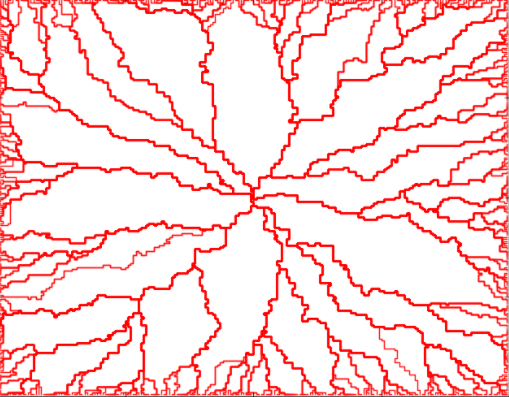
\includegraphics[width=0.45\textwidth]{fpp.png}
   \caption{First passage percolation to the boundary of a lattice graph with exponential edge weights. Figure taken from \cite{wiki}.}
 \end{center}
\end{figure}

Let $G = (V, E, w)$ be a network and suppose $u, v$ are two distinct vertices in $G$.  Let $\xi_e \sim \text{Exponential}(w_e)$. We interpret our weights $w_e$ as the parameters of these random edge traversal times.  The random first passage percolation time from $u$ to $v$, denoted by $X(G)$, is the minimum value of $\sum_{e\in \pi}\xi_e$ over all paths $\pi$ from $u$ to $v$.  Note the that is not necessarily achieved by the path that minimizes $\sum_{e\in \pi}w_e$ since $\xi$ is a random variable so even though some paths may have greater total weight sum, there is still a small probability that the traversal time realization can be smaller than that of a smaller total weight path.  Hence $X(G)$ is a random FPP.  

The functional that interests us in this setting is $$ \Gamma(G) : = \mathbb{E}X(G).$$

Note that to estimate $X(G)$ from the observed process, we actually have two layers of randomness here.  First the randomness contribution from $X(G)$ (which we smooth over with $\mathbb{E}$) and then a contribution from $N_e(t)$, the multi-edges of $G^{obs}$.  

The following lemma gives us an idea of how $X(G^{obs})$ relates to $X(G)$.
In particular to study the functional $\Gamma$ we use the following lemma. 

\begin{lemma}
$$\mathbb{P}(X(G^{obs}(t)) \geq x) \geq \mathbb{P}(X(G) \geq x),\quad 0 < x<\infty .$$
\end{lemma}

Let's tease out why this lemma is phrased in such a way.  For any fixed $t$ we have $\mathbb{P}(X(G^{obs}(t)) = \infty) > 0$ since $v$ and $u$ may not be in the same connected component since the edges arrive as a Poisson process in $G^{obs}$.  Note this is trivially true if $u,v$ not connected, so we are assuming $u$ and $v$ are connected in $G^{true}$.  So estimation procedures should involve the stopping time for when $u$ and $v$ are connected.  The lemma unfortunately does not extend easily to stopping times.  

\begin{proof}
The unconditional distribution of $X(G^{obs}(t))$ is the distribution of FPP times for which edge-traversal times $\xi_e^*(t)$ are independent with distributions given by:\\
the conditional distribution of $\xi_e^*(t)$ given $M_e(t)$ is $ \text{Exponential}(M_e(t)/t)$, where Exponential($a$) denotes the exponential distribution with parameter a. So it is sufficient to show that $\xi^*_e(t)$ stochastically dominates Exponential($w_e$) distribution of $\xi_e$.  

We have

\begin{equation}
\begin{split}
\mathbb{P}(\xi_e^*(t) \geq x) &= \mathbb{E}(\mathbb{P}(\xi_e^*(t) \geq x |N_e(t))\\
&= \mathbb{E}(\exp(-x N_e(t)) \\
&\geq \exp(-x \mathbb{E}(N_e(t)/t))\\
&=\exp(-x w_e)\\
\end{split}
\end{equation}
where the last step follows by Jensen's inequality. 
\end{proof}

\section{A General Conjecture Fails}

Observing $G^{obs}$ will eventually give us a good estimate of $X(G)$, since we can simulate it from $G^{obs}$ once $t$ is large enough that its own FPP process is distributed as $X(G)$. That is, it is clear that 

\begin{equation}
\text{ On every network } G \text{ we require at most } O(\Gamma(G)) \text{ observation time. }
\end{equation}


One may expect however, that for certain types of networks, in particular with a more constrained geometry, we may be able to estimate $\Gamma(G) := \mathbb{E}X(G)$ quicker than having to wait for such a stopping time. Consider the linear graph $G$ as an example.  It is a naturally example since the FPP between edges are much simpler, in fact it is by necessity the path the unique path that connects two nodes. Suppose $G$ has $m$ edges where each edge weight is of order $\Theta(1)$.  Then instead of having to wait for $\Theta(m)$ time in order to , we simply have to wait for $N_e(t)/t$ to be good estimators for $w_e$, which occurs in $\Theta(\log m)$ time (by arguments following from the coupon collector's process).  Another candidate for such an observation time is the following stopping time, inspired from Proposition 3 (section 4.2).  

\begin{equation}
T_k := \inf \{t: M(t) \text{ contains k edge-disjoint paths from } u \text{ to } v\}.
\end{equation}

Where $k$ is large and fixed.  This is a natural candidate since the reason why $\Gamma(G)$ is hard to calculate is because we need to take the infimum over many different paths.  However, a result in this direction is not likely.  Our argument below offers an explanation why.  

\begin{center}
\textbf{Claim:} For any estimator satisfying (5.2), the observation time required must be $\Theta(\Gamma(G))$ for every $G$.  
\end{center}

To see this, let $G_n^{1}$ be a network with $n$ two-edge routes running between vertices $v^*$ and $v^{**}$.  And let the edge weights on all edges in these routes be $n^{-1/2}$.

\begin{figure}
\begin{center}
  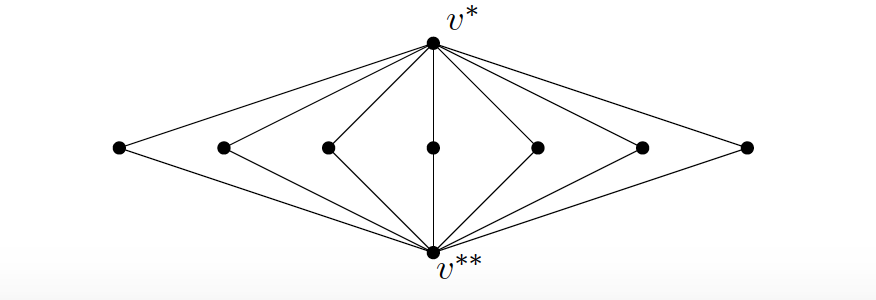
\includegraphics[scale=0.75]{manypaths}
  \caption{Network $G^1_$}
  \label{fig:many_paths}
 \end{center}
\end{figure}



In this case, the observation stopping time defined in 5.3 requires as much time as the FPP time for $\Gamma(G_n^1)$.  Now if we had an estimator that satisfies 5.2, it would have to decide whether to stop at time $t$ or continue observing.  If the decision were based on $M(t)$ it should only use the subset of $M(t)$ that consists of paths from $v^*$ to $v^{**}$.  Suppose by way of contradiction that we have an estimator that requires observation time $\tilde{T}_n << \Gamma(\tilde{G}_n)$.  Let's rescale the edge weights so we can normalize their times so that $\tilde{T}$ is $o(1)$ and $\Gamma(\tilde{G}_n)$ is $\Omega(1)$.  We can now create a new graph $G_n$ which is the union of $\tilde{G}_n$ and $G^1_n$ (by identifying vertices with the same index and taking the union of edges).  Now if we wait $\tilde{T}_n$ time as dictated by graph $\tilde{G}_n$, it will sometimes see the same subset of edges that we would have seen in the case of observing $G^{obs}$ corresponding to $\tilde{G}_n$.  At that point we are in the same empirical position as we would have been if $G^{true}$ were $\tilde{G}_n$, so we would be confident enough to stop observing, as in the case of $\tilde{G}_n$.  However the availability of the many paths to choose from in $G^1_n$ requires that $\Gamma(G_n)$ is in fact $\Theta(1)$.  In other words, we need to observe much longer to get the true min of all passage times. So we we really were incorrect in stopping our observations, since $G$ is a union of $G^1_n$ and $\tilde{G}_n$.  
